\title{Assignment 3.2}
\author{
        Pradyot Prakash - 130050008
            \\
        Utkarsh Mall - 130050037
			\\
		Samarth Mishra - 130260018
}
\date{\today}
\documentclass[11pt]{article}
\usepackage[left=2.5cm,top=2cm,right=2.5cm,bottom=2cm,bindingoffset=0.5cm]{geometry}
\usepackage{graphicx}
\usepackage{siunitx}
\usepackage[section]{placeins}
\graphicspath{ {../images/} }
\renewcommand\thesubsection{(\alph{subsection})}
\begin{document}
\maketitle

\subsection{}
Noise Level for Real and Imaginary components \\
Real Noise Level (found from pixels in imageNoisy(1:50, 1:50)) : 0.060861 \\
Imaginary Noise Level (found from pixels in imageNoisy(1:50, 1:50)) : 0.058865 


\subsection{}
Optimal Values of parameters : \\
Quadratic Prior : $\alpha = 0.8$ \\
Huber Prior : $\alpha = 0.503, \gamma = 0.0424$ \\
Discontinuity-adaptive prior : $\alpha = 0.5, \gamma = 0.23$

\begin{figure}[h]
\centering
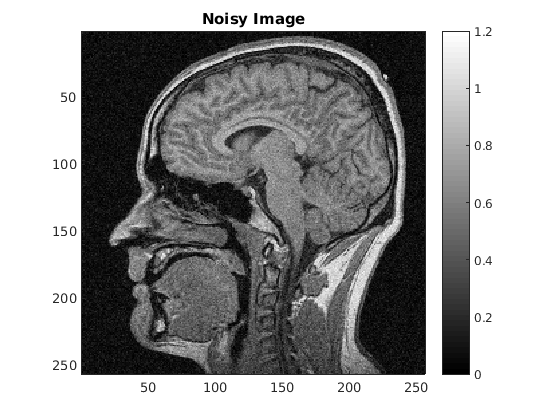
\includegraphics[scale=0.7]{Noisy}
\end{figure}

\begin{figure}[h]
\centering
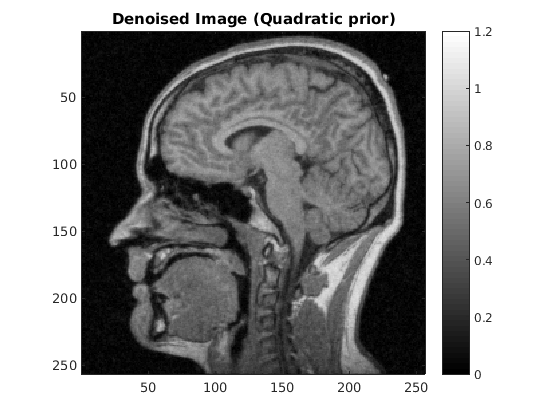
\includegraphics[scale=0.7]{DenoisedQuad}
\end{figure}

\begin{figure}[h]
\centering
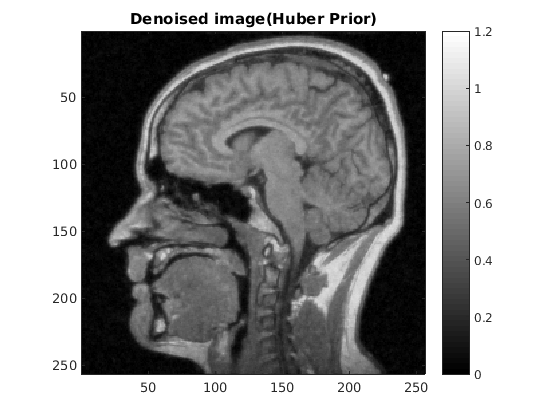
\includegraphics[scale=0.7]{DenoisedHuber}
\end{figure}

\begin{figure}[h]
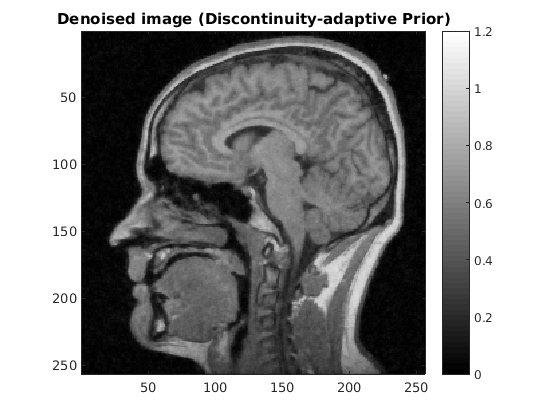
\includegraphics[scale=0.7]{DenoisedDA}
\centering
\end{figure}
\FloatBarrier


\subsection{}
\begin{figure}[h]
\hspace*{-1.5in}
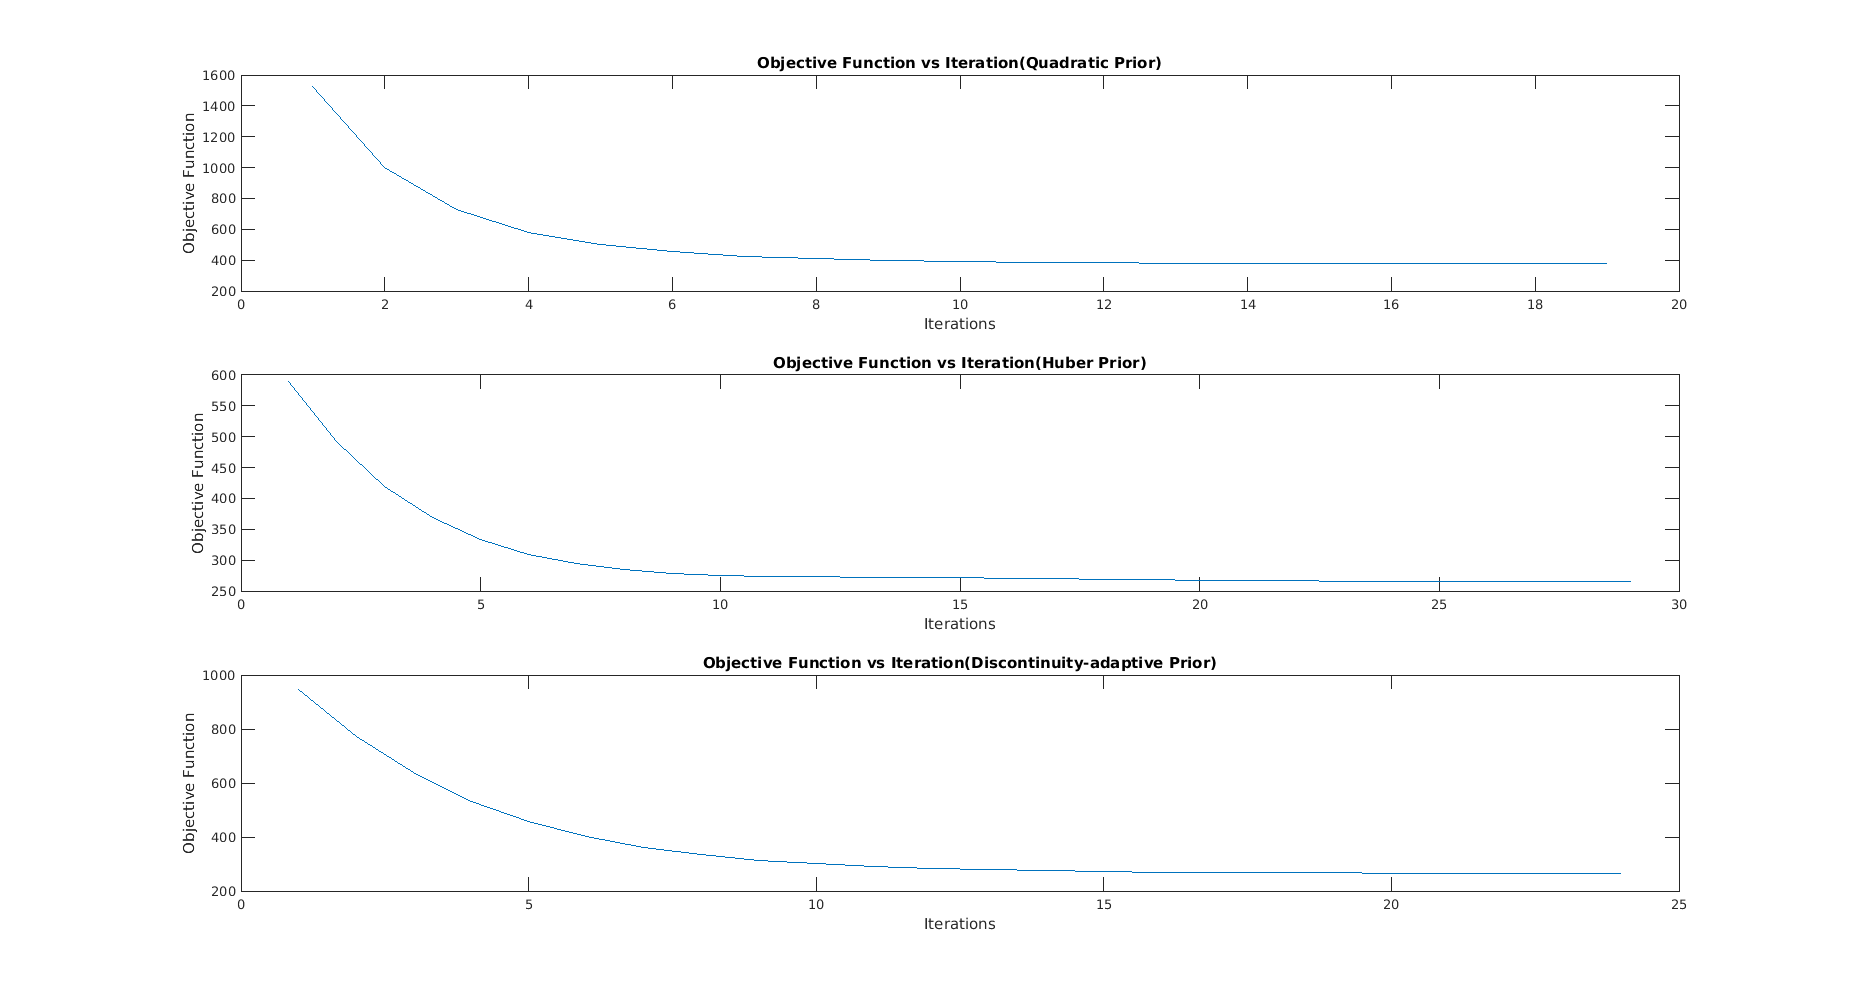
\includegraphics[scale=0.48]{graphs}
\centering
\end{figure}
\FloatBarrier
\end{document}
